\chapter{Estado da Arte}
\label{chap:estadodaarte}

Esta secção tem como objetivo apresentar o estado da arte, analisando um conjunto de ferramentas e/ou produtos que partilham funcionalidades, ou que assentam em modelos de negócio semelhantes ao \textit{Blended4Future}. Em particular, privilegia-se a exploração de plataformas digitais concebidas para a divulgação, gestão e acompanhamento de projetos ou estágios de carácter internacional, onde a colaboração entre instituições, empresas e estudantes assume um papel central.

Para além de identificar soluções com finalidades comparáveis, pretende-se também realçar as suas principais características distintivas, apontando os pontos fortes, limitações e contextos de utilização.

\section{ESN - \textit{European Student Network}}

A Erasmus Student Network (ESN) é uma organização sem fins lucrativos fundada em 1989 e atualmente presente em mais de 40 países europeus. O seu objetivo principal é apoiar e enriquecer a experiência de estudantes em mobilidade internacional, nomeadamente no âmbito do programa Erasmus+, mas também de outros programas de intercâmbio académico e profissional. Através de uma vasta rede de secções locais, a ESN promove atividades culturais, sociais e profissionais que favorecem a integração dos estudantes nos países de acolhimento.

Para além das suas atividades presenciais, a ESN tem desenvolvido várias plataformas digitais que servem de apoio à comunidade estudantil, oferecendo acesso a informações sobre oportunidades de estágio, bolsas de estudo, e até serviços de voluntariado internacional. Estas ferramentas constituem um importante meio de ligação entre estudantes, instituições e empresas, permitindo assim fomentar uma experiência de mobilidade mais completa e enriquecedora.

\subsection{erasmusintern.org}

Dentro da ampla rede de iniciativas desenvolvidas pela Erasmus Student Network (ESN), destaca-se particularmente o projeto \textit{ErasmusIntern.org}, que constitui o departamento dedicado à divulgação de oportunidades de estágio em formato online.

\begin{figure}[h!tbp]
    \centering
    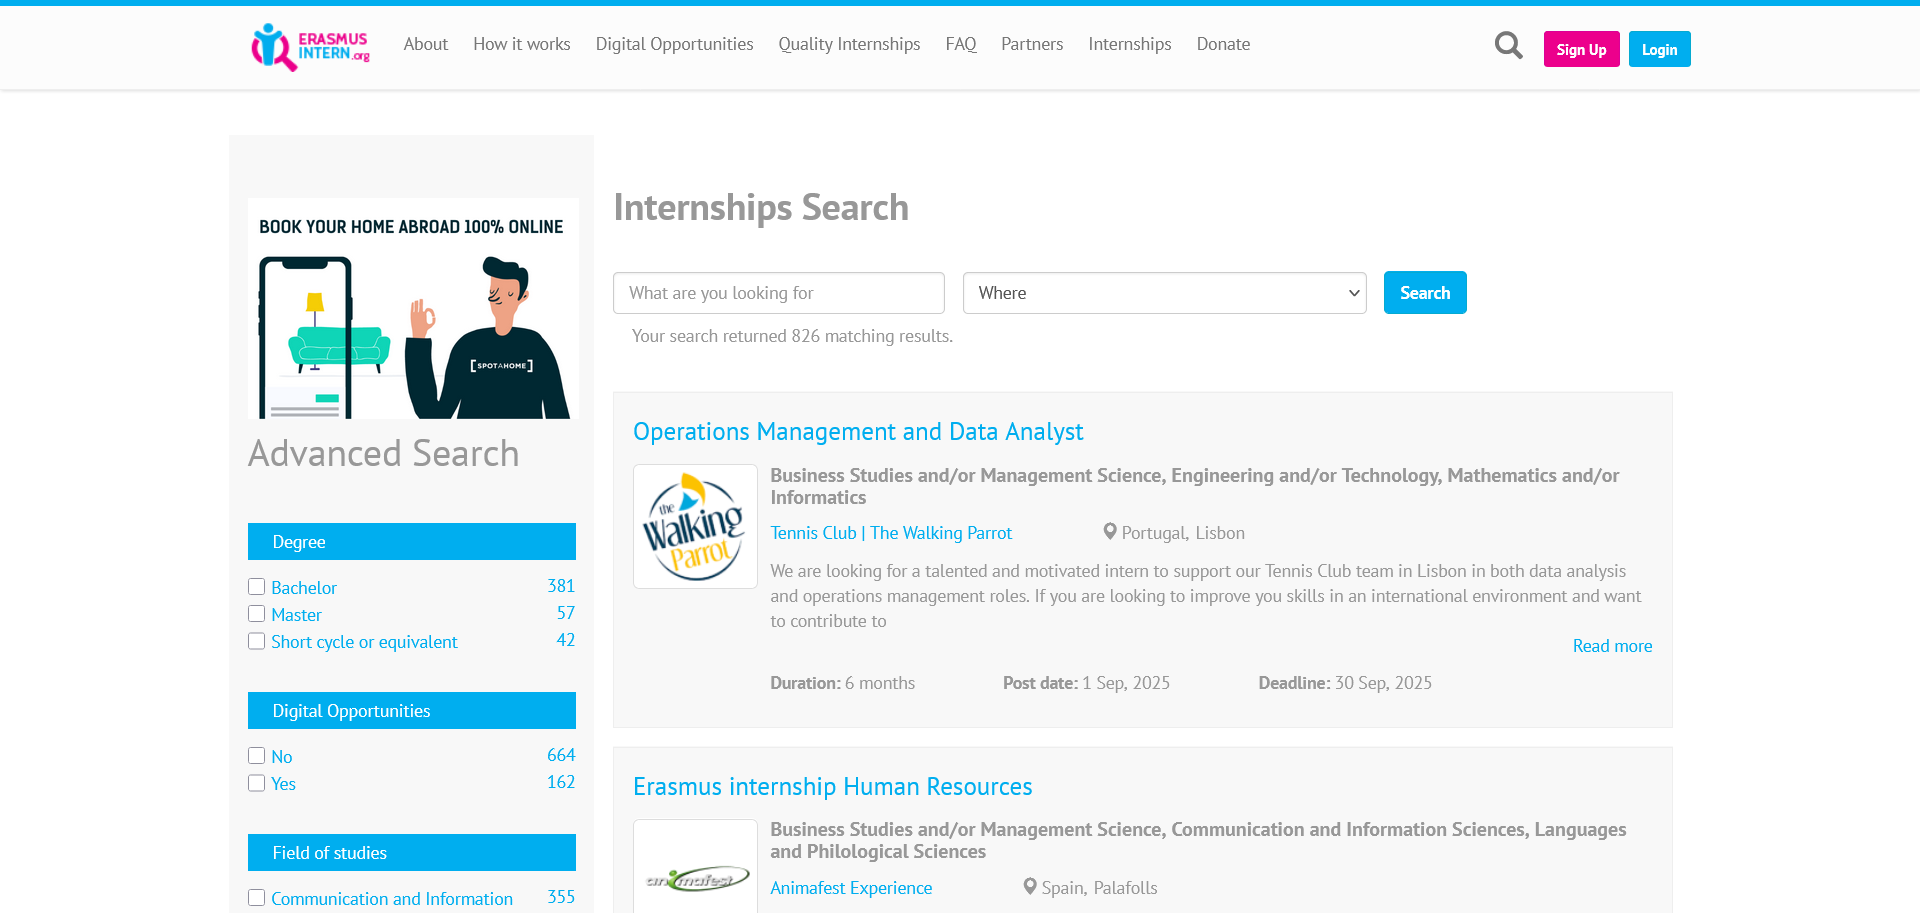
\includegraphics[width=\linewidth]{capitulos/cap2-estadodaarte/assets/image/esn/internship-org.png}
    \caption{Website do erasmusintern.org}
    \label{fig:erasmus-intern-org}
\end{figure}

Num contexto desta natureza, em que a diversidade académica e cultural dos utilizadores é extremamente elevada, a disponibilização de mecanismos de pesquisa eficazes assume um papel central. A existência de filtros específicos, nomeadamente por área de estudo, setor de atividade, localização geográfica ou duração do estágio, torna-se fundamental para garantir que os estudantes encontram rapidamente as oportunidades que melhor correspondem ao seu perfil e às suas expectativas.

\begin{figure}[h!tbp]
    \centering
    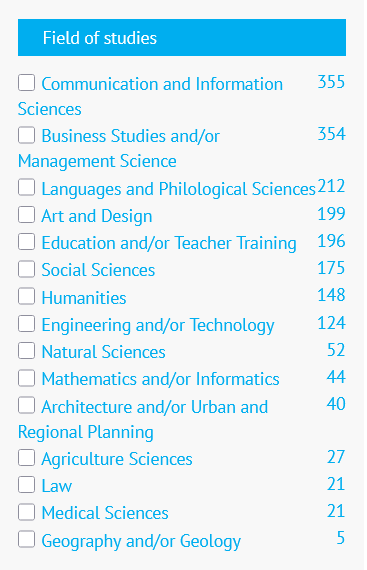
\includegraphics[width=0.3\linewidth]{capitulos/cap2-estadodaarte/assets/image/esn/erasmus-intern filters.png}
    \caption{Filtros de pesquisa divididos por \textit{Area de Estudo} do erasmusintern.org}
    \label{fig:erasmus-intern-org}
\end{figure}

\section{Plataforma de estágios PRAXIS}

Também conhecida como \textit{praxisnetwork.eu}, esta plataforma apresenta uma função bastante semelhante à desempenhada pela \textit{ErasmusIntern.org}, centrando-se igualmente na promoção e intermediação de estágios internacionais para estudantes universitários. A PRAXIS Network resulta de uma colaboração entre diversas instituições de ensino superior europeias, procurando criar uma rede sólida que facilite a mobilidade estudantil e, simultaneamente, aumente a cooperação entre universidades e entidades empregadoras.

\begin{figure}[h!tbp]
    \centering
    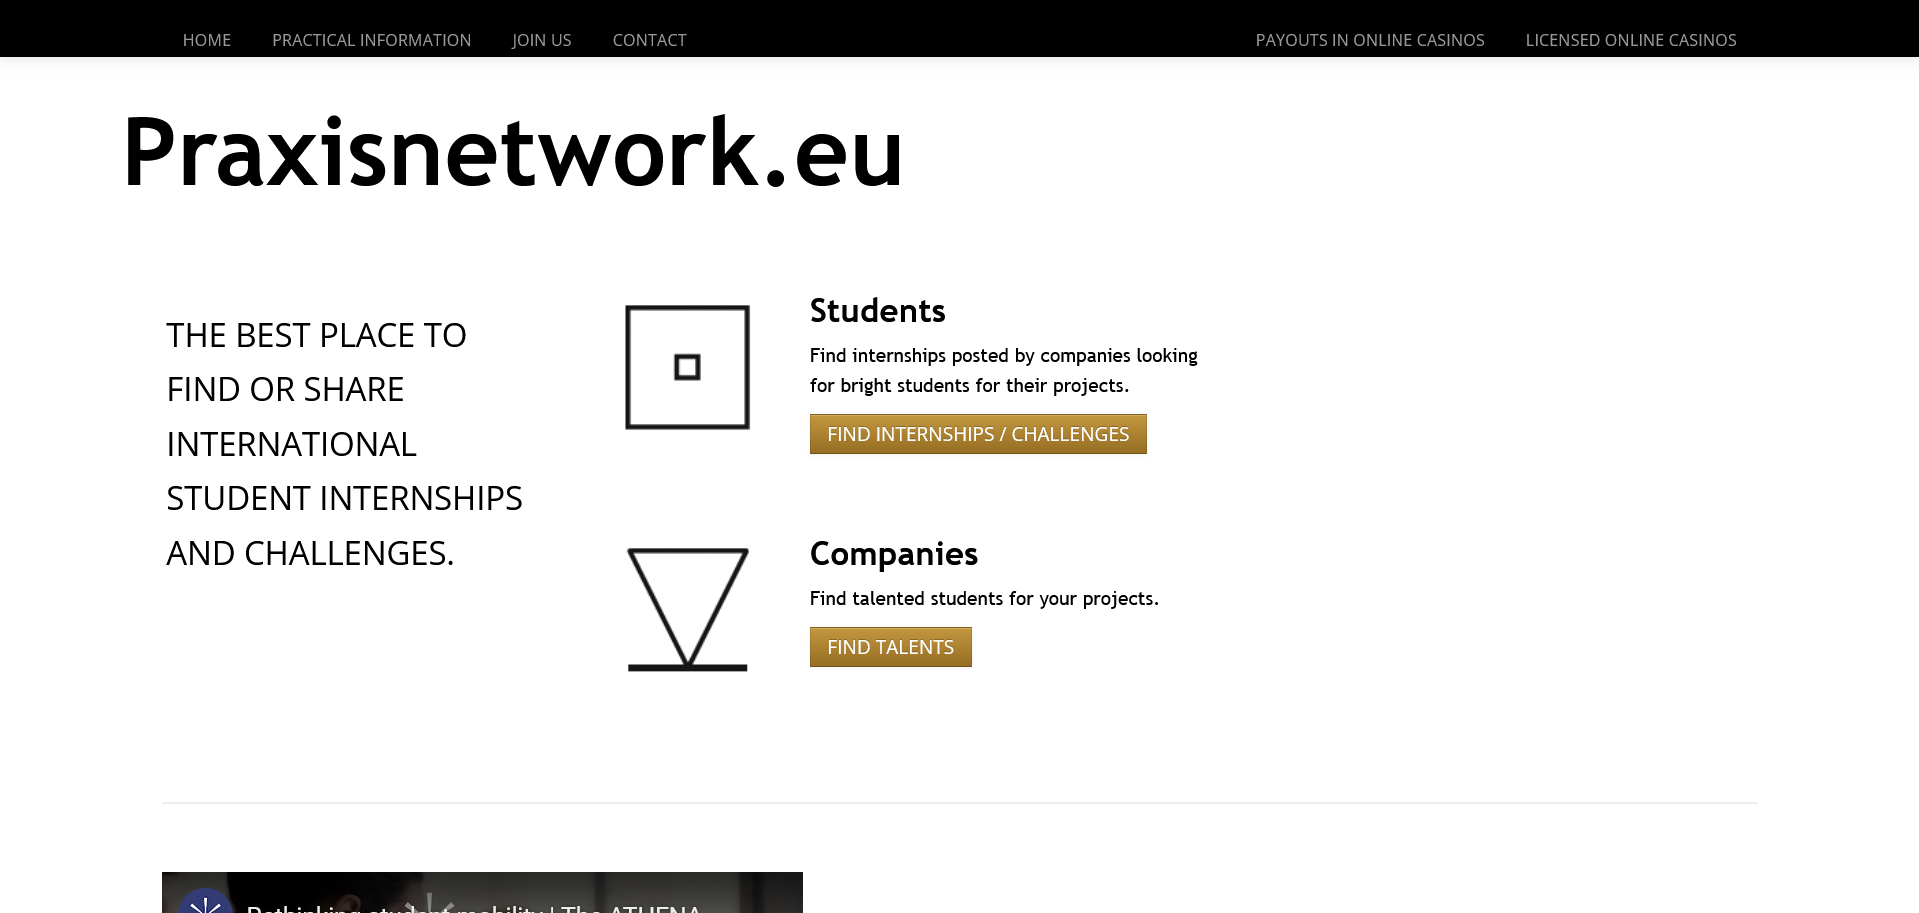
\includegraphics[width=\linewidth]{capitulos/cap2-estadodaarte/assets/image/praxis/praxis-home-page.png}
    \caption{\textit{Home page} da praxisnetwork.eu}
    \label{fig:erasmus-intern-org}
\end{figure}

\section{\textit{Spain Internship}}